% -*-coding: utf-8-*-
% This is an AMS-LaTeX v. 1.2 File.

\documentclass{report}

%\usepackage{pscyr}
%\renewcommand{\rmdefault}{fjn}
%\renewcommand{\ttdefault}{fcr}

%\usepackage{showkeys}
\usepackage[T2A]{fontenc}
\usepackage[utf8x]{inputenc}
\usepackage[english,russian]{babel}
\usepackage{expdlist}
\usepackage[dvips]{graphicx}
\usepackage{amsmath}
\usepackage{amssymb}
\usepackage{amsthm}
\usepackage{amsfonts}
\usepackage{amsxtra} 
\usepackage{sty/dbl12}
\usepackage{srcltx}
\usepackage{epsfig}
\usepackage{verbatim}
\usepackage{sty/rac}
%\usepackage[russian]{sty/ralg}
\usepackage{listings}


%%%%%%%%%%%%%%%%%%%%%%%%%%%%%%%%%%%%%%%%%%%%%%%%%%%%%%%%%%%%%%%%%%%%%%%%%%%%%%

% Redefine margins and other page formatting

\setlength{\oddsidemargin}{0.5in}

% Various theorem environments. All of the following have the same numbering
% system as theorem.

\theoremstyle{plain}
\newtheorem{theorem}{Теорема}
\newtheorem{prop}[theorem]{Утверждение}
\newtheorem{corollary}[theorem]{Следствие}
\newtheorem{lemma}[theorem]{Лемма}
\newtheorem{question}[theorem]{Вопрос}
\newtheorem{conjecture}[theorem]{Гипотеза}
\newtheorem{assumption}[theorem]{Предположение}

\theoremstyle{definition}
\newtheorem{definition}[theorem]{Определение}
\newtheorem{notation}[theorem]{Обозначение}
\newtheorem{condition}[theorem]{Условие}
\newtheorem{example}[theorem]{Пример}
\newtheorem{algorithm}[theorem]{Алгоритм}
%\newtheorem{introduction}[theorem]{Introduction}

\renewcommand{\proof}{\\\textbf{Доказательство.}~}

%\def\startprog{\begin{lstlisting}[language=Java,basicstyle=\normalsize\ttfamily]}

%\theoremstyle{remark}
%\newtheorem{remark}[theorem]{Remark}
%\include{header}
%%%%%%%%%%%%%%%%%%%%%%%%%%%%%%%%%%%%%%%%%%%%%%%%%%%%%%%%%%%%%%%%%%%%%%%%%%%%%%%

\numberwithin{theorem}{chapter}        % Numbers theorems "x.y" where x
                                        % is the section number, y is the
                                        % theorem number

%\renewcommand{\thetheorem}{\arabic{chapter}.\arabic{theorem}}

%\makeatletter                          % This sequence of commands will
%\let\c@equation\c@theorem              % incorporate equation numbering
%\makeatother                           % into the theorem numbering scheme

%\renewcommand{\theenumi}{(\roman{enumi})}

%%%%%%%%%%%%%%%%%%%%%%%%%%%%%%%%%%%%%%%%%%%%%%%%%%%%%%%%%%%%%%%%%%%%%%%%%%%%%%


%%%%%%%%%%%%%%%%%%%%%%%%%%%%%%%%%%%%%%%%%%%%%%%%%%%%%%%%%%%%%%%%%%%%%%%%%%%%%%%

%This command creates a box marked ``To Do'' around text.
%To use type \todo{  insert text here  }.

\newcommand{\todo}[1]{\vspace{5 mm}\par \noindent
\marginpar{\textsc{ToDo}}
\framebox{\begin{minipage}[c]{0.95 \textwidth}
\tt #1 \end{minipage}}\vspace{5 mm}\par}

%%%%%%%%%%%%%%%%%%%%%%%%%%%%%%%%%%%%%%%%%%%%%%%%%%%%%%%%%%%%%%%%%%%%%%%%%%%%%%%

\binoppenalty=10000
\relpenalty=10000

\begin{document}


\bibliographystyle{sty/gost71s}       % Set the bibliography style to AMS
                                % alphabetized. (Can use ``amsalpha'' or
                                % ``abbrv''instead.)

% Begin the front matter as required by Rackham dissertation guidelines

\initializefrontsections

\pagestyle{title}

\begin{center}
Санкт-Петербургский национальный исследовательский университет \\ информационных технологий, механики и оптики

\vspace{2cm}

Кафедра компьютерных технологий

\vspace{3cm}

{\Large А. К. Касс}

\vspace{2cm}

\vbox{\LARGE\bfseries
Массовая задача определения кратчайшего расстояния\\до произвольной
конфигурации отрезков на плоскости}

\vspace{4cm}

Бакалаврская работа 

\vspace{1cm}

{\Large Научный руководитель: А. С. Ковалев}

\vspace{6cm}

Санкт-Петербург\\ 2012
\end{center}

\newpage

\setcounter{page}{2}
\pagestyle{plain}

%\dedicationpage{Put a dedication here}
% Dedication page

%\startacknowledgementspage
% Acknowledgements page
%{Put Acknowledgements here}

% Table of contents, list of figures, etc.
\tableofcontents
%\listoffigures


\def\t#1{\mbox{\texttt{\hbox{#1}}}}
\def\b#1{\textbf{#1}}
\def\tb#1{\t{\b{#1}}}

\def\cln#1{\t{#1}}
\def\pcn#1{\t{#1}}
\newcommand{\p}{\par Здесь будет текст...}

\def\drawfigure#1#2#3{
        \begin{figure}[H]
        \centerline{ \includegraphics{pic/#1}}
        \caption{#2}
        \label{#3}
        \end{figure}
}
\def\drawfigurex#1#2#3#4#5{
        \begin{figure}[#1]
        \centerline{ \includegraphics[#2]{#3}}
        \caption{#4}
        \label{#5}
        \end{figure}
}

% Chapters
\startthechapters
% -*-coding: utf-8-*-
%$\newcommand{\ncs}{\mbox{N-CROSS} SUM}
%\newcommand{\threecs}{\mbox{3-CROSS} SUM}
%\newcommand{\fourcs}{\mbox{4-CROSS} SUM}
%\newcommand{\sat}{\mbox{1-in-3 SAT}}
%\newcommand{\six}{$(A, B, a_0, b_0, s, V)$}
%\newcommand{\tdld}{\mbox{2-DLD}}
%\newcommand{\false}{\t{КНФЭ}}
%\newcommand{\true}{\t{ХЯРХМЮ}}
%\newcommand{\gadget}{\ttfamily}
%\newcommand{\setA}{$\mathcal A_1$}
%\newcommand{\setB}{$\mathcal A_2$}
%\newcommand{\setC}{$\mathcal A_2'$}

\startprefacepage

Задача определения кратчайшего расстояния до конфигурации отрезков
(dist2segments), являясь частным случаем задачи dist2sites -- задачи о
минимальном расстоянии до произвольного набора линейных данных,
является одной из базовых задач вычислительной геометрии (computational
geometry) \cite{PrSh}. На решении данной задачи базируются решения некоторых задач
об избежании столкновений (collision avoidance problem) \cite{MarNav}, некоторых задачи
из области геоинформационных систем (Geographic information system, GIS) \cite{CGinGIS},
текстурирования рельефа, математического моделирования движения твердых
тел в жидкости и многих других.

Очень часто возникает необходимость в достаточно
больших количествах запросов на поиск ближайших отрезков.
Например, такая необходимость возникает при расчете физики движения судов в морских
тренажерах \cite{MarNav}. Судов может быть достаточно много, объектов, с которыми
необходимо рассчитать взаимодействие тоже достаточно много. Это означает,
что запросы расстояний до ближайших отрезков идут достаточно часто, чтобы это стало проблемой
для ЭВМ, вычислительная мощность которых может быть недостаточно
большой для такого потока данных. Такого рода запросы называются
массовыми запросами, а такая задача -- массовой задачей.

Массовая задача в \cite{PrSh} определена следующим образом: существует
фиксированный набор входных данных $S$. Требуется вычислить массовый
запрос $Q$, то есть ответить на некоторый поставленный вопрос для каждого
запроса из $Q$. Иногда такие задачи решаются в два этапа – предобработка 
(pre-processing) и вычисление запросов на некоторой структуре данных,
формирующейся на этапе предобработки и облегчающей поиск, что позволяет
сократить суммарное время по сравнению с последовательным решением
исходной задачи для каждого запроса.
Логично предположить, что такая структура данных должны быть
подобна хешу (hash) \cite{AHU} или дереву (tree) \cite{QT, SQT, FANN}. В работе \cite{NGRID} была предложена
такая структура данных -- многоуровневая сеть (n-grid). Если потребовать,
чтобы с каждой ячейкой сети ассоциировались только ближайшие к этой
ячейке отрезки, то задача сводится к перебору небольшого числа отрезков. В
данной работе будет рассмотрена древовидная структура -- квадродерево,
позволяющая наиболее эффективно решать массовые геометрические задачи
такого типа, и методы ее построения, а также будет произведено сравнение
этой структуры с многоуровневой сетью и явным построением диаграммы
Вороного.
Вообще, задача определения кратчайшего расстояния до конфигурации
отрезков имеет очевидное решение -- это полный
перебор с отсечением, имеющий линейную сложность ($O(n)$) \cite{DnCG}. Однако, если
множество точек-запросов $Q$ имеет достаточно большую мощность, обычно
рассматривают так называемую диаграмму Вороного для отрезков (segment
Voronoi diagram, SVD) \cite{PrSh, CGAL}. Эта структура данных похожа на диаграмму
Вороного для точек (point Voronoi diagram) \cite{PrSh, CGAL}, однако она не может быть
представлена реберным списком с двойными связями (double-connected edge
list, DCEL, РСДС) \cite{PrSh, CGAL} в силу своей нелинейности. Хотя, конечно, можно
создать приближенный РСДС, сколь угодно точно описывающий диаграмму
Вороного для отрезков.

%%-*-coding: utf-8-*-
\chapter{Shortest path from one vertex to every other}


\FloatBarrier
\section{Classic sequential Bellman-Ford}

\FloatBarrier
\begin{algorithm}
\caption{Classic Bellman-Ford}\label{bf_classic_seq}
\begin{algorithmic}[1]
\Procedure{ClassicBellmanFord}{$G,start$}
\State {$dist \gets \left\{ {\infty ... \infty}\right\}$}
\State {$dist[start] \gets 0$}
 
\For{$i = 0$ to $|G.vertices| - 1 $}
	\For{$e \in G.edges $}
		\State $dist[e.to] \gets \min(dist[e.to], dist[e.from] + e.w)$
	\EndFor
\EndFor
\State \textbf{return} $dist$
\EndProcedure
\end{algorithmic}
\end{algorithm}

\FloatBarrier
\section{BFS-like sequential Bellman-Ford}

\FloatBarrier
\begin{algorithm}
\caption{BFS-like BellmanFord}\label{bf_bfs_seq}
\begin{algorithmic}[1]
\Procedure{BFSBellmanFord}{$G,start$}
\State $dist\gets \left\{ {\infty ... \infty}\right\}$
\State $dist[start] \gets 0$
\State $CurrentVertexSet \gets \left\{ {start}\right\}$\Comment{Set of vertices the distance to which has just been updated} 
\State $NextVertexSet \gets \emptyset$ 
\State {$step \gets 0$ }
\While {$step < |G.vertices|$ \algorithmicand \algorithmicnot $ CurrentVertexSet.empty()$}
	\State $step \gets step + 1$
	\State $NextVertexSet.clear()$
	
	\For{$v \in CurrentVertexSet$}
		\For{$e \in G.edgesFrom[v] $} \Comment{Outgoing edges of current vertex} 
			\If {$dist[e.to] < dist[e.from] + e.w$} 
				\State $dist[e.to] \gets dist[e.from] + e.w$
				\State $NextVertexSet.insert(e.to)$								
			\EndIf
		\EndFor
	\EndFor
	
	\State $CurrentVertexSet \gets NextVertexSet$	
\EndWhile
\State \textbf{return} $dist$

\EndProcedure
\end{algorithmic}
\end{algorithm}


\FloatBarrier
\subsection{Parallel Bellman-Ford by edges of current vertex}
Idea : use parallel min reduce for incoming edges of current vertex   


\FloatBarrier
\begin{algorithm}
\caption{Parallel Bellman-Ford by edges of current vertex}\label{bf_classic_par1}
\begin{algorithmic}[1]
\Procedure{BellmanFordPar1}{$G,start$}
\State $dist\gets \left\{ {\infty ... \infty}\right\}$
\State $dist[start] \gets 0$
 
\For{$i = 0$ to $|G.vertices| - 1 $}
	\State {$changed \gets $ \algorithmicfalse}
	\For{$v \in G.vertices $}
		\algrenewcommand\algorithmicfor{\textbf{parfor}}
		\State {$minDist \gets $ min reduce by G.inEdges[v]} 
		
		\If {$dist[v] > minDist$} 
			\State $dist[v] \gets minDist$
			\State {$changed \gets $ \algorithmictrue}						
		\EndIf
		\algrenewcommand\algorithmicfor{\textbf{for}}

	\EndFor
	\If {\algorithmicnot $changed$} 
		\State $break$
	\EndIf
\EndFor
\State \textbf{return} $dist$
\EndProcedure
\end{algorithmic}
\end{algorithm}

\FloatBarrier
\subsection{Parallel Bellman-Ford by all edges using prefixsum}

Idea : use precalculated prefixsum to divide current vertex set for 2 sets, which will be handled by different threads


\FloatBarrier
\begin{algorithm}
\caption{Parallel Bellman-Ford by all edges using prefixsum}\label{bf_classic_par2}
\begin{algorithmic}[1]
\Procedure{BellmanFordPar2}{$G,start$}
\State $dist\gets \left\{ {\infty ... \infty}\right\}$
\State $dist[start] \gets 0$
\State {$prefsum \gets $ prefix sum by vertices incoming degree} 
\State {$planMap \gets $ \Call {BuildPlan}{$prefsum$, 0, |$G.vertices$|}} 

\For{$i = 0$ to $|G.vertices| $}	
	\If {\algorithmicnot \Call {ProcessLayer}{$G, planMap, prefsum, 0, |G.vertices|$}} 
		\State \textbf{break}
	\EndIf
		
\EndFor
\State \textbf{return} $dist$
\EndProcedure

\State 
\Procedure{BuildPlan}{$prefsum, startV, endV$}  \Comment{This function returns a structure which tells us the middle of the segments (by index of start and end vertex)}
\State {$resultMap \gets $ empty map}
\State $edgesNumber \gets prefsum[endV] - prefsum[startV]$
\If {$edgesNumber < threshold$} 
	\State $midV \gets $ binary search by edges number
	\State $resultMap[startV][endV] \gets midV$ 
	\State {$resultMap.addAll($ \Call {BuildPlan}{$prefsum, startV, midV$})} 
	\State {$resultMap.addAll($ \Call {BuildPlan}{$prefsum, midV, endV$})} 
\EndIf

\State \textbf{return} $resultMap$
\EndProcedure

\State 
\Procedure{ProcessLayer}{$G, planMap, prefsum, startV, endV$}  
\State $edgesNumber \gets prefsum[endV] - prefsum[startV]$
\If {$edgesNumber < threshold$} 
	\State process vertices sequentally 	
\Else	
	\State $midV \gets planMap[startV][endV]$ 
	\State {\Call {ProcessLayer}{$G, planMap, prefsum, startV, midV$}}
	\State {\Call {ProcessLayer}{$G, planMap, prefsum, midV, endV$}}
\EndIf

\EndProcedure

\end{algorithmic}
\end{algorithm}

\FloatBarrier
\subsection{Parallel BFS-like Bellman-Ford}
Idea : use your PBFS to handle vertex distances

\FloatBarrier
\begin{algorithm}
\caption{Parallel BFS-like Bellman-Ford}\label{bf_bfs_par}
\begin{algorithmic}[1]
\Procedure{BellmanFordPar3}{$G,start$}
\State $dist\gets \left\{ {\infty ... \infty}\right\}$
\State $dist[start] \gets 0$
\State {$Frontier \gets \left\{ {G.edgesFrom(start)}\right\}$}
\For{$i = 0$ to $|G.vertices| $}	
	\State {$Frontier \gets $  {\Call {HandleFrontier}{$Frontier$}}} \Comment{relax edges from Frontier and build a new one} 
	
	\If { $Frontier.empty()$} 
		\State $break$						
	\EndIf
		
		
\EndFor
\State \textbf{return} $dist$
\EndProcedure
\State
\Procedure{HandleFrontier}{$Frontier$}
\State recursively divide current frontier, atomically relax edges in frontier and building a new one

\State \textbf{return} $NewFrontier$
\EndProcedure

\end{algorithmic}
\end{algorithm}


\FloatBarrier
\subsection{Algo comparison}
At the first sight it may seems that Algorithm 3 has only disadvantages. The main problem is that it has bad parallelisation ability compared to other two algorithms. But sometimes it works better even on 40-core machine because of one useful property. Let's consider a graph where all the edges have the from $i \rightarrow j$ where $i < j$. Once the iteration number $I$ has passed all the vertices till $I$ have correct target distance. It' easy to prove using mathematic induction. So it means that we have to perform only 2(!!!) loops in that case. One for calculating distance and one for understanding that nothing will change anymore. And let's assume that we have a dense graph. In that circumstances Algorithm 4 will suffer from great parallelism (the number of iterations of the main loop will increase significantly) and Algorithm 5 will have to handle the large set of vertices (because graph is dense) during the iterations. 

But anyway it's easy to see that in the most cases Algorithm 4 and Algorithm 5 will beat Algorithm 3. Let's compare them. As I said before Algorithm 5 will be not good enough when we're considering dense graphs, because of big size of queue. So the main recommendation of when to use these approaches is to realise if the graph is dense or sparse. In the first case you have to use Algorithm 4, otherwise Algorithm 5.


\FloatBarrier
\subsection{Testing}

Now we'll prove our assumptions on practice. I've implemented all the algorithms and compared them. Description of input graphs is presented in the Table 1.1. The results are presented in the Table 1.2
\FloatBarrier

\begin{table}[H]
\centering

\begin{tabular}{c|c|c}  
Name & Vertices & Edges\\
\hline\hline
CompleteTS sign(-) & 7071 & 24995985 \\  
Complete sign & 3162 & 9995082  \\  
BalancedTree fraction & 8388607 & 8388608 \\  
SquareGrid sign & 2499561 & 4999122  \\  
RandomSparse fraction(0.5) sign & 2500000 & 25000000  \\  
RandomSparse fraction(0.96) sign(+) & 2500000 & 25000000  \\  
RandomDense fraction(0.5) sign & 5000 & 25000000  \\  
RandomDense fraction(0.96) sign(+) & 5000 & 25000000  \\  
\hline
\multicolumn{3}{l}{\footnotesize \textit{sign} - sign of weights on edges }\\
\multicolumn{3}{l}{\footnotesize \textit{fraction} - fraction of lexicographically sorted edges (edges of type X -> X+i) }\\
\multicolumn{3}{l}{\footnotesize \textit{TS} - exists only Lexicographically Sorted edges (fraction = 1) }\\
\multicolumn{3}{l}{\footnotesize }\\
\multicolumn{3}{l}{\footnotesize  expression "\textit{RandomDense fraction(0.5) sign}" means Random Dense }\\
\multicolumn{3}{l}{\footnotesize 	graph with specified fraction and any sign of weights}\\
\end{tabular}

\caption{Input graph description}
\label{bf_algo_comparison}
\end{table}
\FloatBarrier

\begin{table}[H]
\centering

\begin{tabular}{l|ccc|cc|cc|ccc|ccc}  
Algo №& \multicolumn{3}{c}{Complete} & \multicolumn{2}{c}{BalancedTree} & \multicolumn{2}{c}{SquareGrid} & \multicolumn{3}{c}{RandomSparse} & \multicolumn{3}{c}{RandomDense}\\
& TS- & + & - & 0.5 & 1 & + & +- & 0.5+  & 0.5- & 0.96+ & 0.5+ & 0.5- & 0.96+\\
\hline\hline
3 & 2.43 & 4.65 & nc & 116.31 & 9.04 & 5.49 & 13.40 & nc & nc & 24.35 & nc & nc & 5.01 \\  
4 & 5.17 & 0.18 & 10.84 & 3.59 & 3.08 & 5.92 & 7.10 & 2.77 & 14.68 & 2.42 & 0.48  & 6.38  & 0.46 \\
5 & 44.63 & 0.37 & 23.55 & 0.44 & 0.31 & 4.42 & 0.58 & 0.98 & 22.59 & 0.76  & 0.60  & 10.25 & 0.71 \\
\hline
\end{tabular}

\caption{Bellman-Ford algorithms comparison}
\label{graph_description}
\end{table}

\FloatBarrier
\section{Conclusion}

You can easily find out from tables that our assumptions were correct. Algorithm 3 works good for dense graph with very high fraction (almost 1), Algorithm 4 is good for dense graphs and for graphs with negative edges, Algorithm 5 is good for sparse graph with positive edges. 

\FloatBarrier

%%-*-coding: utf-8-*-
\chapter{Решение задачи поиска расстояний между каждой парой вершин графа}

В этой главе будет приведено решение задачи поиска расстояний между каждой парой вершин. В начале главы будет краткий обзор предметной области, далее будут приведены два решения для поиска искомых расстояний, а после будет приведено решение задачи для социальных неориентированных невзвешенных графов, которое будет сочетать в себе несколько подходов и идей, изложенных в предыдущих алгоритмах. 

\FloatBarrier
\section{Обзор существующих решений}

\subsection{Алгоритм Флойда}
Одним из наиболее известных алгоритмов, который применяется для решения данной задачи является алгоритм Флойда. Этот алгоритм использует идею динамического программирования и выполняется за $O(V^3)$. Основная идея состоит в обновлений пути между двумя текущими вершинами выбором некоторой вершины, через которую может пройти потенциальный кратчайший путь. Псевдокод алгоритма приведен ниже. 

\FloatBarrier
\begin{algorithm}
\caption{Алгоритм Флойда}\label{floyd}
\begin{algorithmic}[1]
\Procedure{Floyd}{$G$}
\State $dist\gets \left\{ {   \left\{ {\infty \ldots \infty}\right\}  \ldots \left\{ {\infty \ldots \infty}\right\} }\right\}$
\For{$e \in G.edges $}
	\State $dist[e.from][e.to] \gets e.w$
\EndFor 
\State
\For{$i = 0$ to $|G.vertices| $}
	\For{$u = 0$ to $|G.vertices| $}
		\For{$v = 0$ to $|G.vertices| $}
			\State $dist[u][v] \gets \min(dist[u][v], dist[u][i] + dist[i][v])$
		\EndFor
	\EndFor
\EndFor
\State \textbf{return} $dist$
\EndProcedure
\end{algorithmic}
\end{algorithm}

\FloatBarrier
\subsection{Альтернативы}
В некоторых случаях оказываются эффективны другие подходы. Например, можно для каждой вершины по отдельности запустить некоторый алгоритм поиска кратчайшего пути до всех остальных вершин. Для случая неотрицательных ребер можно применить алгоритм Дейкстры, в более общем случае может быть применен Беллман-Форд. Кроме вышеприведенных подходов также известен алгоритм Джонсона, который работает на графах без циклов отрицательного веса и находит кратчайшие расстояния за время $O(V^2 \log(V) + VE)$. Все эти алгоритмы оказываются эффективны в случае разреженных графов.

В последующих подходах в качестве основы для параллельного алгоритма будет использоваться именно идея подсчета расстояний либо для каждой вершины по отдельности, либо подсчета расстояний для групп вершин одновременно. И все нижеперечисленные алгоритмы, как и описанные выше альтернативы, хорошо работают на разреженных графах.

\FloatBarrier
\section{Наивная параллельная версия}
Первая версия заключается исключительно в запуске Беллмана-Форда для каждой из вершин. При этом заметим, что так как каждый из них независим друг от друга, то можем эти запуски распараллелить между собой. В качестве простого критерия остановки разделения множества для обработки будем использовать некоторую константу $threshold$. Кроме того, важно отметить, что необходимо выбирать наиболее подходящую реализацию параллельного Беллмана-Форда в зависимости от типа графа. К примеру, в случае разреженного графа с положительными ребрами нам подойдет последняя реализация, основанная на параллельном обхода в ширину. Таким образом, псевдокод из себя представляет следующее.


\FloatBarrier
\begin{algorithm}
\caption{Наивная параллельная версия}\label{all_pairs_par1}
\begin{algorithmic}[1]
\Procedure{AllPairsPar1}{$G$}
\State \textbf{return} {\Call {HandleVertices}{$G, 0, |G.vertices|$}}
\EndProcedure
\State
\Procedure{HandleVertices}{$G, startVertex, endVertex$}

\If {$endVertex - startVertex < threshold$} 
	\State $distances \gets$ Запустить параллельную версию Беллмана-Форда для каждой вершины из полуинтервала $[startVertex, endVertex)$ 
	\State \textbf{return} $distances$	
\Else	
	\State $midVertex \gets (startVertex + endVertex) / 2$ 
	\State \begin{varwidth}[t]{\linewidth}fork2(\par
        \hskip\algorithmicindent {\Call {HandleVertices}{$G, startVertex, midVertex$}},\par
        \hskip\algorithmicindent {\Call {HandleVertices}{$G, midVertex, endVertex$}});
      \end{varwidth}
	
\EndIf

\EndProcedure

\end{algorithmic}
\end{algorithm}

\FloatBarrier
\section{Параллельный алгоритм для объединенного графа}
Развитием предыдущей идеи является наблюдение, что для некоторого набора вершин можем построить общий граф и запустить на нем Беллмана-Форда, что потенциально может повысить производительность за счет высокой параллельности для общего графа, в то время как для каждого отдельно взятого Беллмана-Форда она низкая. Кроме того, это избавит нас от выбора константы для предыдущей версии, что упростит использование алгоритма для пользователя. 

Идея заключается в запуске алгоритма Беллман-Форд на графе, вершины которого описываются двумя значениями - текущей вершины в обходе и вершины, из которой этот обход начался (иными словами, вершины, из которой мы ищем кратчайшие расстояния). После построения графа будет достаточно запустить обход, при этом положив в Frontier все вершины вида $(i, i)$. В итоге кратчайшее расстояние для вершины $(i, j)$ будет интерпретироваться как кратчайшее расстояние от вершины $i$ до вершины $j$ в исходном графе. Описанный алгоритм иллюстрирован на примере простейшего графа из 3 вершин на рисунке \ref{floyd_par_common_graph}. 
\FloatBarrier

\begin{figure}[h]
\caption{Пример преобразования для простейшего графа}
\label {floyd_par_common_graph}
\centering
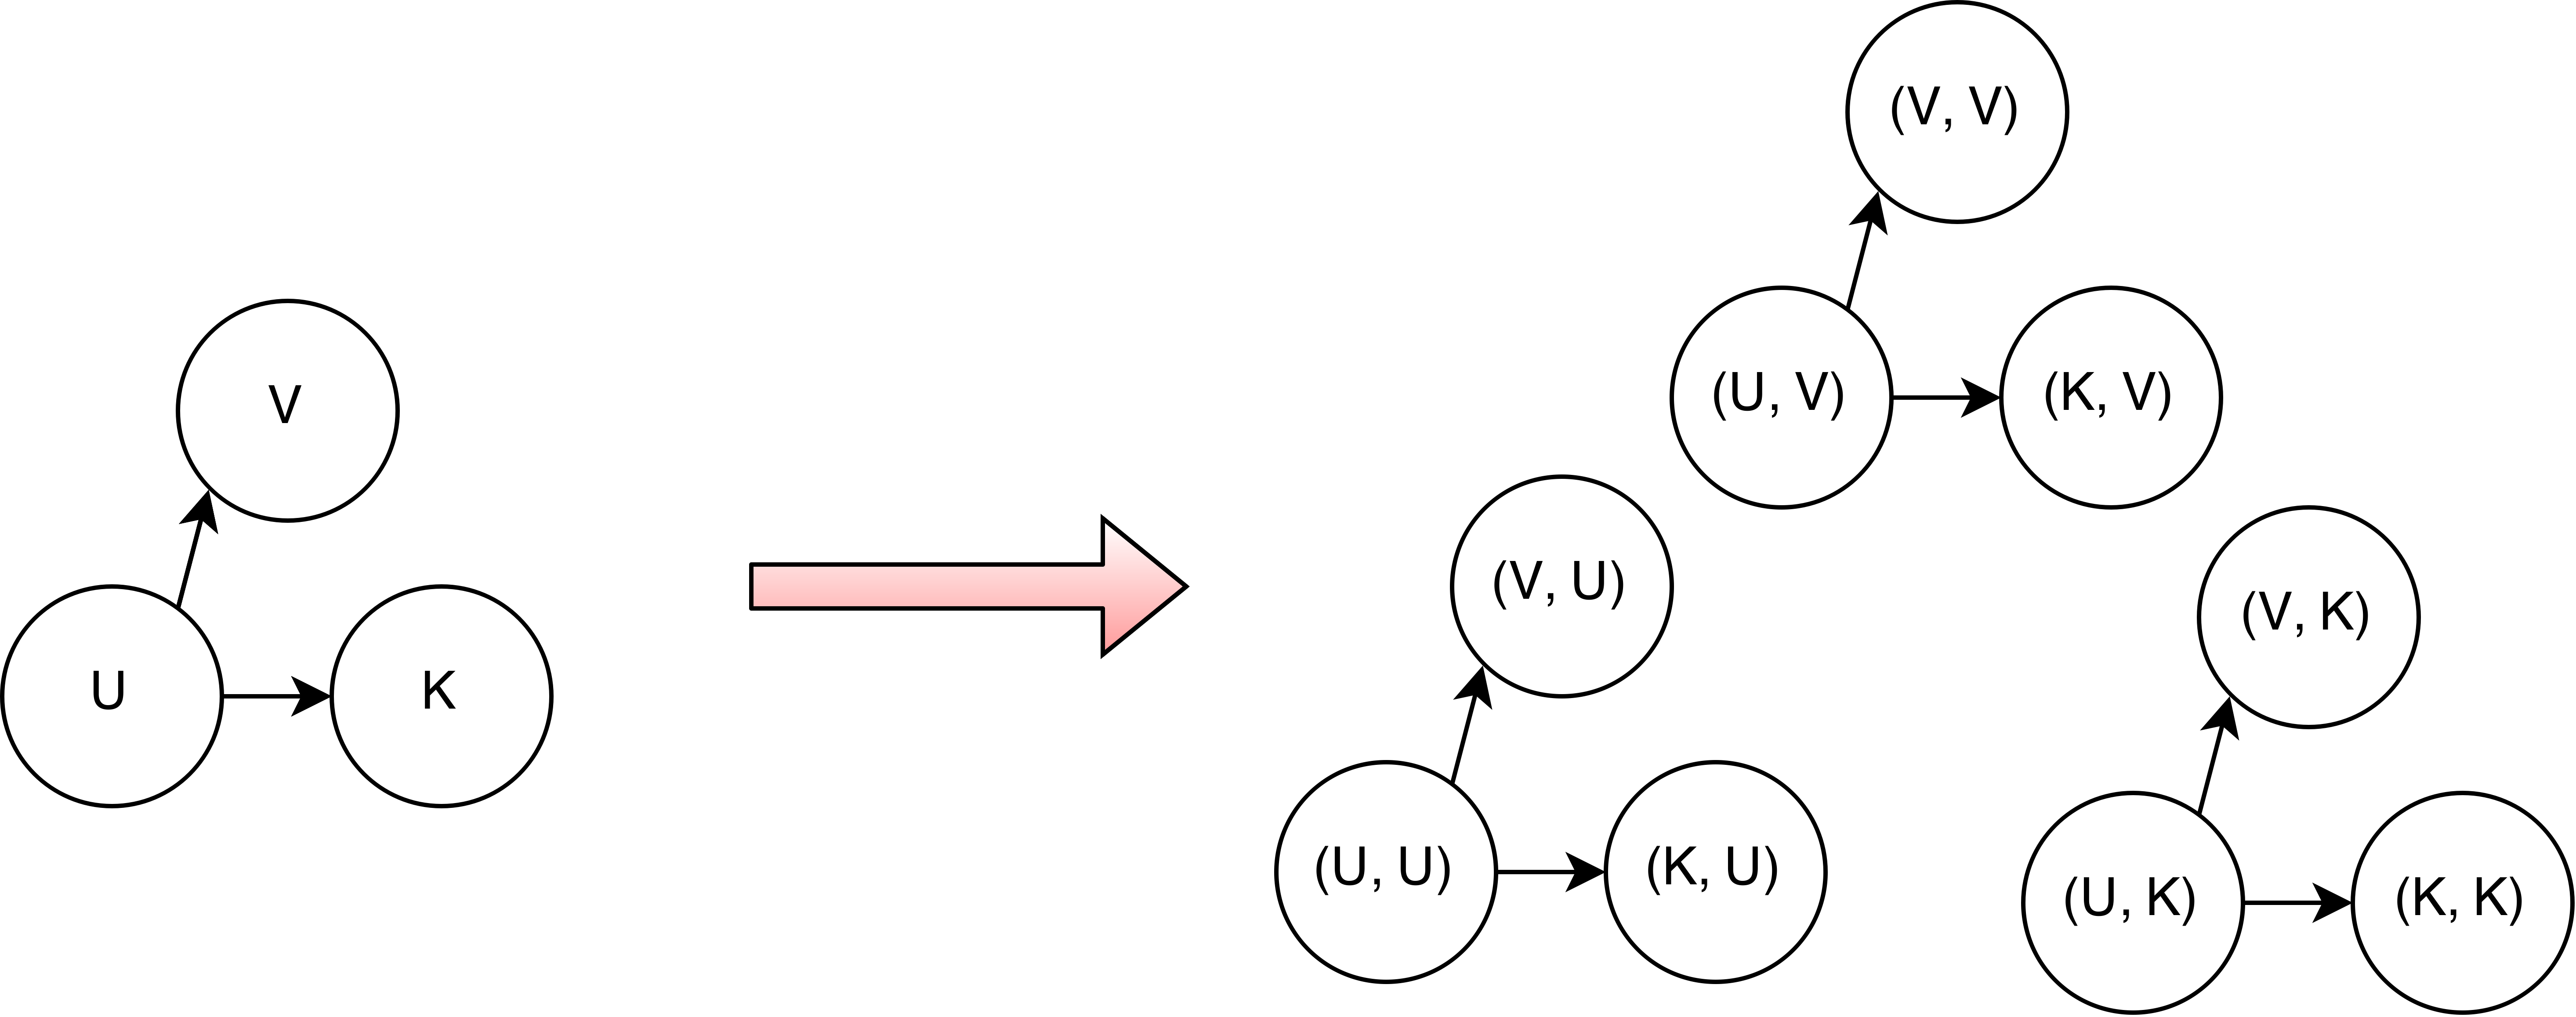
\includegraphics[width=0.9\textwidth]{img/floyd_par_2.png}
\end{figure}
\FloatBarrier

Однако, как будет показано позднее, такой подход на практике оказался немного медленнее наивной версий. Но при этом идея обработки ряда вершин одновременно легла в основе следующего алгоритма для социальных графов. 
\FloatBarrier
\section{Параллельный алгоритм для социальных графов}
В данном разделе будет рассмотрен алгоритм поиска кратчайшего пути между каждой парой вершин для графов реальных социальных сетей. При этом рассмотренный граф будет невзвешенный и неориентированный. Кроме того, в этой главе будет рассмотрена производительность алгоритма на примере реальных подграфов известных социальных сетей, таких как Twitter и Slashdot\cite{STANFORDGRAPHS}.

\FloatBarrier
\subsection{Идея алгоритма}
В графах для социальных сетей известна одна эвристика, которая называется "Теория шести рукопожатий". В ее основе лежит тот факт, что практически любые два человека на земле знакомы не более, чем через пятерых промежуточных людей. Таким образом, выбрав некоторую случайную вершину, мы сможем добраться от нее до большинства других вершин не более, чем за 6 ребер. Воспользуемся этой эвристикой в нашем алгоритме и выберем вершину наибольшей степени в качестве базовой. И рассмотрим два множества - вершины, которые находятся на расстоянии не более 6 от базовой ("большое" множество) и все остальные вершины ("меньшее" множество). Кроме того, будем обрабатывать эти два множества различным образом - для меньшего будем запускать параллельного Беллмана-Форда для каждой вершины, для большого - воспользуемся методом динамического программирования для подсчета ответа. Пример разбиения социального графа на два эти множества проиллюстрирован на рисунке \ref{floyd_social}. Рассмотрим более подробно принцип работы алгоритма.

\begin{figure}[h]
\caption{Пример разбиение социального графа на 2 множества}
\label {floyd_social}
\centering
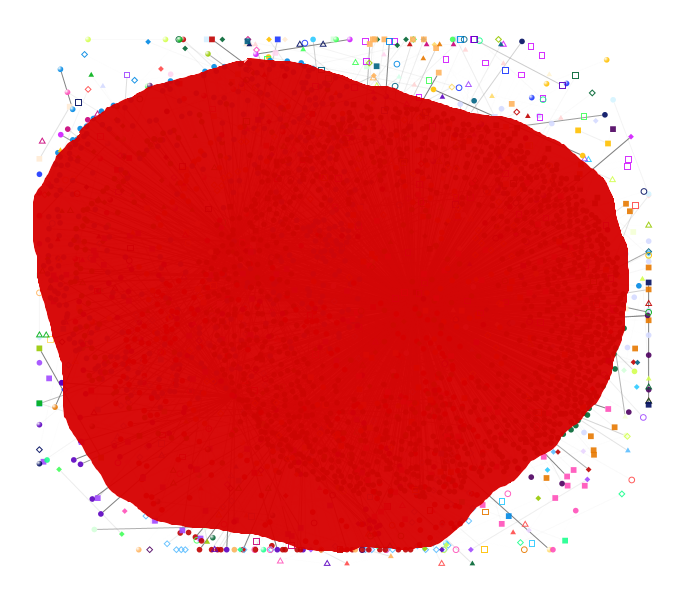
\includegraphics[width=0.9\textwidth]{img/floyd_social.png}
\end{figure}
\FloatBarrier

\FloatBarrier
\subsection{Работа алгоритма}
Как уже было отмечено ранее, работа алгоритма разбивается на три этапа, которые в дальнейшем будут рассмотрены по отдельности.

\begin{itemize}
  \item Анализ графа и выбор базовой вершины. 
  \item Обработка меньшего множества параллельным Беллманом-Фордом.
  \item Обработка большего множества методом динамического программирования
\end{itemize}

Первый и самый простой этап состоит в выборе базовой вершины. В качестве нее будет выбрана вершина с наибольшей степенью. После этого из этой вершины будет запущен обход в ширину, который найдет все вершины, отстоящие не более, чем на $K$ (в случае классической теории шести рукопожатий $K = 6$). Таким образом, все такие вершины попадают в большее множество $handleByBaseVertexSet$, которое будет обработано на третьем этапе алгоритма. Все остальные вершины попадают в меньшее множество $otherVertexSet$. Псевдокод этого этапа выглядит следующим образом

\FloatBarrier
\begin{algorithm}
\caption{Первая фаза алгоритма}\label{all_pairs_social1}
\begin{algorithmic}[1]
\Procedure{ConstructSets}{$G$}
\State {$baseVertex \gets $ Вершина максимальной степени}
\State {$dist \gets $ Запустить обход в ширину из $baseVertex$}
\State $handleByBaseVertexSet \gets \emptyset$
\algrenewcommand\algorithmicfor{\textbf{parfor}} 
\For{$i = 0$ to $|G.vertices| - 1$}
\algrenewcommand\algorithmicfor{\textbf{for}}
	\If {$dist[i] \leq K$ }
		\State $handleByBaseVertexSet.add(i)$
	\EndIf
\EndFor

\State $otherVertexSet \gets G.vertices \setminus handleByBaseVertexSet$
\State $otherVertexSet \gets otherVertexSet \cup  \left\{ {baseVertex}\right\}$
 
\State \textbf{return} $ baseVertex, handleByBaseVertexSet, otherVertexSet$
\EndProcedure

\end{algorithmic}
\end{algorithm}




В качестве алгоритма для обработки второго множества запустим параллельный обход в ширину (он же Беллман-Форд) для каждой из вершин этого множества. Иными словами, мы просто воспользуемся Алгоритмом 7 для множества вершин (для $otherVertexSet$). При этом исходя из наших эвристик мы предполагаем небольшие размеры множества, что позволяет думать об этом этапе как о значительно менее затратным по времени по сравнению с последним. Кроме того, значения расстояния, посчитанные обходом в ширину из базовой вершины нам помогут на третьем этапе, поэтому добавим в множество $otherVertexSet$ базовую вершину (чтобы в дальнейшем при обращений к глобальному массиву $dist$ в нем содержались корректные расстояния от базовой вершины).

Для поиска искомых значении для вершин множества $handleByBaseVertexSet$ воспользуемся методом динамического программирования. Но сперва обсудим основные принципы построения алгоритма и доказательство его корректности. 

Рассмотрим некоторую вершину, которая находится на расстояний $d$ от базовой вершины ($d \leq K$). То какие вершины для нее могут находится на расстоянии $i$? Это могут быть только те вершины, которые находятся на расстоянии $[i-d, \ i+d]$ от базовой. Иначе бы не выполнялось свойство, что путь кратчайший. С другой стороны, если рассмотреть некоторую вершины, расстояние до которой от базовой равняется $i$, то для всех вершин из множества $handleByBaseVertexSet$ верно, что кратчайшее расстояние от них до нее варьируется в промежутке $[i-K, \ i+K]$. 

 Предположим, что мы запустили обход в ширину из всех вершин большого множества. То какие вершины могут быть в слое с номером $i$? Ответ вытекает из рассуждений предыдущего абзаца - только вершины, расстояние от которых до базовой варьируется в промежутке $[i-K, \ i+K]$. То есть каждая из вершин будет принимать участие в не более, чем $2K+1$ слоях. То построим для каждого слоя обхода в ширину множество возможных вершин на этом слое. Это избавит нас от построения таких множеств в процессе работы алгоритма. И при этом общее количество вершин во всех слоях будет пропорционально числу вершин в графе (если учитывать, что $K$ - небольшое число, меньшее 7). 
 
 После того, как мы построили набор вершин для каждого из слоев мы можем воспользоваться структурой данных Frontier для эффективного распараллеливания процесса обработки ребер, исходящих из этих вершин. Однако к текущему моменту мы никак не воспользовались тем фактом, что вершины расположены близко друг к другу, и, может быть, существует эффективный технических прием для оптимальной обработки группы вершин. Такой подход существует и основан на идее динамического программирования и применения битовых векторов (bitset). Обратим внимание, что битовые вектора должны поддерживать битовые логические операции (конъюнкция, дизъюнкция и отрицание) и стандартные методы установки соответствующего бита и его получение.
 
 Будем поддерживать две следующие динамики. Значениями в полях массива будут битовые вектора --- это некоторая структура, где каждый из битов соответсвует вершине из множества $handleByBaseVertexSet$. 
 
 \begin{itemize}
  \item $mask[u][i]$ --- набор вершин, расстояние от которых до $u$ равно $i$ 
  \item $calc[u][i]$ --- набор вершин, расстояние от которых до $u$ меньше $i$
\end{itemize}
 
 Рассмотрим процесс пересчета значений динамики. Для подсчета текущего значения $mask[v][i]$ воспользуемся формулой (2.1). Суть формулы состоит в переборе всех ребер графа, входящих в текущую вершину и применение операции битовое "или" для соответствующих масок. При этом мы не должны учитывать данные для тех вершин, расстояние до которых уже посчитано (эта информация хранится в массиве $calc$).  
  
%mask[v][i] = \bigvee (mask[u][i - 1] where \exists edge u->v) AND (

\FloatBarrier
\begin{equation}
mask[v][i] = \neg calc[v][i - 1] \wedge \bigvee_{\exists (u, v) \in E} mask[u][i - 1] 
\end{equation}
\FloatBarrier

В свою очередь $calc$ пересчитывается согласно (2.2)
\FloatBarrier
\begin{equation}
calc[v][i] = calc[v][i - 1] \vee mask[v][i]
\end{equation}
\FloatBarrier

Псевдокод пересчета значений динамики представлен ниже. Обратим внимание, что для каждой вершины нам достаточно хранить всего $2K + 1$ битовых векторов. Однако для упрощения понимания псевдокода будем обращаться к $i$ слою вершины $u$ просто как $mask[u][i]$, при этом имея в виду эту значительную оптимизацию по памяти. Кроме того другим важным замечанием является то, что когда нам необходимо посчитать значения динамики для слоя $i$, то нам необходимо обрабатывать предыдущий слой. Таким образом в последнем цикле алгоритма для обработки $layerToCalc$ мы используем $frontierLayer \gets layerToCalc - 1$.

\FloatBarrier
\begin{algorithm}
\caption{Пересчет динамики}\label{all_pairs_social2}
\begin{algorithmic}[1]
\State $ K \gets 6$ \Comment{Максимальная глубина до базовой вершины}\ldots
\State

\Procedure{CalculateDistancesForBigSet}{$G, baseVertex, handleByBaseVertexSet$}
\State {$maxLayer \gets $ calculate max distance from baseVertex}
\State {$Frontiers \gets \left\{ {Frontier_0 \ldots Frontier_{maxLayer + K}}\right\} $} \Comment{Фронтир для каждого уровня обхода} 
\State {$VertexSets \gets \left\{ {VertexSet_0 \ldots VertexSet_{maxLayer + K}}\right\} $} \Comment{Набор вершин для каждого уровня} 
\State $mask\gets \left\{ {   \left\{ {bitVector(0) \ldots bitVector(0)}\right\}  \ldots \left\{ {bitVector(0) \ldots bitVector(0)}\right\} }\right\}$ 
\State $calc\gets \left\{ {   \left\{ {bitVector(0) \ldots bitVector(0)}\right\}  \ldots \left\{ {bitVector(0) \ldots bitVector(0)}\right\} }\right\}$
\State

\For{$i = 0$ to $maxLayer + K$}	
	\For{$j = dist[baseVertex][i] - K$ to $dist[baseVertex][i] + K$}		
		\State $Frontiers[j].pushEdgesOf(i)$
		\State $VertexSets[j].addVertex(i)$
	\EndFor
\EndFor
\State

\For{$v \in handleByBaseVertexSet $}
	\State $mask[v][0] \gets bitVector(bitNum(v))$ \Comment{Будем считать, что существует функция bitNum, которая по номеру вершины возвращает соответсвующий ей бит} 

\EndFor 
\State
\For{$layerToCalc = 1$ to $maxLayer + K$}
	\State $frontierLayer \gets layerToCalc - 1$ 
	\State {\Call {ProcessLayerLazy}{$G, Frontiers[frontierLayer], mask, layerToCalc$}}

	\algrenewcommand\algorithmicfor{\textbf{parfor}}
	\For{$v \in VertexSets[layerToCalc] $}
		\State {$calc[v][layerToCalc] \gets mask[v][layerToCalc] $}
		\If {$layerToCalc$ is not first layer for vertex $v$}
			\State $calc[v][layerToCalc - 1] \gets \lnot calc[v][layerToCalc - 1]$ 
			\State $mask[v][layerToCalc] \gets mask[v][layerToCalc] \land calc[v][layerToCalc - 1]$ 
			\State $calc[v][layerToCalc - 1] \gets \lnot calc[v][layerToCalc - 1]$ 
			\State $calc[v][layerToCalc] \gets calc[v][layerToCalc] \lor calc[v][layerToCalc - 1]$ 
		\EndIf

	\EndFor 
	\algrenewcommand\algorithmicfor{\textbf{for}}	
\EndFor 
\EndProcedure
\end{algorithmic}
\end{algorithm}
\FloatBarrier

Для полноты алгоритма осталось описать обработку текущего Frontier. Псевдокод этого этапа представлен ниже. В этом алгоритме мы снова (как и в алгоритмах из первой главы) пользуемся интерефейсом, который предоставляет библиотека для параллельных вычислений PASL. Напомню, что для взаимодействие между рабочими потоками существует служебные функции, дающие понять потокам необходимость разбиения фронтира для обработки на других ядрах или же понять обратное. 
\begin{algorithm}
\caption{Обработка Фронтира}\label{all_pairs_social3}
\begin{algorithmic}[1]

\Procedure{ProcessLayerLazy}{$G, Frontier, mask, layer, dists, baseVertex$}
\While {\algorithmicnot $Frontier.empty()$}
	\If {$hasIncomingQuery()$}
		\If {$Frontier.nbEdges() \leq cutoff$}
			\State $rejectQuery()$			
		\Else		
			\State $NewFrontier \gets \emptyset$
			\State $Frontier.split(NewFrontier)$
			\State \begin{varwidth}[t]{\linewidth}fork2(\par
        \hskip\algorithmicindent {\Call {ProcessLayerLazy}{$G, Frontier, mask, layer, dists, baseVertex$}},\par
        \hskip\algorithmicindent {\Call {ProcessLayerLazy}{$G, NewFrontier, mask, layer, dists, baseVertex$}});
      \end{varwidth}
		\EndIf
		
	\EndIf
	\State Frontier.iterNumber(pollingCutoff, updateFunction(mask, from, to, layer, dists, baseVertex))
\EndWhile
\EndProcedure
\State
\Procedure{UpdateFunction}{$mask, from, to, layer, dists, baseV$}
\If {HaveOnLayer(layer - 1, from, dists, baseV) \algorithmicand HaveOnLayer(layer, to, dists, baseV)} 
	
	\State $mask[to][layer] \gets mask[to][layer] \lor mask[from][layer - 1]$ \Comment Атомарно
\EndIf
\EndProcedure
\State
\Procedure{HaveOnLayer}{$layer, vertex, dists, baseV$}
\State \textbf{return} {$|layer - dists[baseV][vertex]| \leq K$}  
\EndProcedure

\end{algorithmic}
\end{algorithm}


\FloatBarrier
Наконец, как по имеющимся данным динамики восстановить ответ? Для каждого значения $mask[u][i]$ найдем единичные биты в маске. Установленный в единицу бит $j$ говорит о том, что расстояние от вершины из "большого" множества с идентификатором $j$ до вершины $u$ равно $i$. Таким образом, мы сможем полностью восстановить ответ для каждой вершины. 

Важным замечанием к коду является последовательность выполнения циклов в последней части алгоритма. Рассмотрим на примере как происходит обращение к памяти в двух различных вариантах (Алгоритм \ref{fill_way_1} и Алгоритм \ref{fill_way_2}), при этом выполняющих совершенно одно и то же. Заметим, что в этих алгоритмах отличается порядок параллельных циклов. 

\FloatBarrier
\begin{algorithm}
\caption{Заполнение массива ответа по динамика (1 вариант)}\label{fill_way_1}
\begin{algorithmic}[1]

\Procedure{FillDistances1}{$G, dist, mask, baseVertex, handleByBaseVertexSet$}
\algrenewcommand\algorithmicfor{\textbf{parfor}}
\For{$v = 0$ to $|G.vertices|$}
\algrenewcommand\algorithmicfor{\textbf{for}}
	\For{$j = dist[baseVertex][i] - K$ to $dist[baseVertex][i] + K$}	
		\algrenewcommand\algorithmicfor{\textbf{parfor}}	
		\For{$u \in handleByBaseVertexSet$}
			\If {$mask[v][j].getBit(bitNum(u)) = 1$}
				\State $dist[u][v] = j$		
			\EndIf	
		\EndFor
		\algrenewcommand\algorithmicfor{\textbf{for}}
	\EndFor
\EndFor 
\EndProcedure
\end{algorithmic}
\end{algorithm}

\FloatBarrier
\begin{algorithm}
\caption{Заполнение массива ответа по динамика (2 вариант)}\label{fill_way_2}
\begin{algorithmic}[1]

\Procedure{FillDistances2}{$G, dist, mask, baseVertex, handleByBaseVertexSet$}
\algrenewcommand\algorithmicfor{\textbf{parfor}}
\For{$u \in handleByBaseVertexSet$}
\algrenewcommand\algorithmicfor{\textbf{for}}
	\For{$j = dist[baseVertex][i] - K$ to $dist[baseVertex][i] + K$}	
		\algrenewcommand\algorithmicfor{\textbf{parfor}}	
		\For{$v = 0$ to $|G.vertices|$}
			\If {$mask[v][j].getBit(bitNum(u)) = 1$}
				\State $dist[u][v] = j$		
			\EndIf	
		\EndFor
		\algrenewcommand\algorithmicfor{\textbf{for}}
	\EndFor
\EndFor 
\EndProcedure
\end{algorithmic}
\end{algorithm}
\FloatBarrier

Так как некоторый $mask[i][j]$ представляет из себя область последовательной памяти, то в случае первого варианта процессор будет работать при вызове методов $getBit$ именно с последовательной памятью, в то время как вторая версия будет обращаться к различным элементам матрицы $mask$ и тем самым к разным участками памяти, что, заметно медленнее в силу специфик устройства вычислительной машины. Это замечание было подтверждено и на практике - алгоритм со второй реализаций работает (на той же машине, которая упоминалась в контексте тестирования параллельного Беллмана-Форда) в среднем в 1.5 раза дольше, чем с первым вариантом.

Итого, псевдокод алгоритма выглядит следующим образом.

\FloatBarrier
\begin{algorithm}
\caption{Параллельная версия для социальных графов}\label{all_pairs_social}
\begin{algorithmic}[1]

\Procedure{AllPairsSocialPar}{$G$}
\State $dist\gets \left\{ {   \left\{ {\infty \ldots \infty}\right\}  \ldots \left\{ {\infty \ldots \infty}\right\} }\right\}$
\State {$ baseVertex, handleByBaseVertexSet, otherVertexSet \gets ConstructSets(G)$}
\State {\Call {AllPairsPar1}{$G, otherVertexSet, dist$}} \Comment {Наивный алгоритм для множества вершин}
\State {\Call {CalculateDistancesForBigSet}{$G, baseVertex, otherVertexSet, dist$}}
\State {\Call {FillDistances1}{$G, dist, mask, baseVertex, handleByBaseVertexSet$}}
\State \textbf{return} $dist$ 
\EndProcedure

\end{algorithmic}
\end{algorithm}


\FloatBarrier
\subsection{Сравнение с другими алгоритмами}

В контексте задачи поиска кратчайших расстояний между каждой парой вершин существует множество подходов. Однако заметим, что для социальных графов наш алгоритм дает асимптотически наилучшее время. Поскольку он работает за $O(VE)$, а в графе социальной сети, как видно в таблице \ref{table:algo_floyd_avg_vertex_degree}, средняя степень вершины ограничена константой около 200, то можем считать, что количество ребер в графе асимптотически равно $O(V)$. Таким образом, наш алгоритм будет работать за $O(V^2)$. Таким образом, множественные подходы, которые опираются на перемножение матриц (например, предложенный Рэймондом Сейделем \cite{SEIDEL}) и имеют в своей асимптотике некоторую степенную функцию от количества вершин, будут асимптотически хуже нашего алгоритма. Обратим внимание, однако, что наивная версия алгоритма, представленная в начале главы, будет асимптотически эквивалентна параллельному алгоритму для социальных графов. Однако, алгоритм для социальных графов имеет ряд преимуществ по сравнению с наивной версией. 


\begin{itemize}
  \item Пересчет расстояний для группы вершин выполняется быстрее за счет битовых операций. Хоть это и не сказывается на асимптотику, но на практике дает заметный выигрыш. 
  \item Все битовые операции выполняются без выделения дополнительной памяти. При этом изменяются уже созданные поля в массиве для подсчета динамики
  \item Так как каждый из фронтиров уже построен, то нам не приходится строить следующий фронтир по предыдущему в процессе обработки
  \item Каждый из получившихся фронтиров довольно большой, что увеличивает его способность к параллелизации
  \item Все остальные этапы также хорошо параллелятся
\end{itemize}

\begin{table}[H]
\centering

\begin{tabular}{l|c}  
Социальная сеть & Средняя степень вершины\\
\hline\hline
Facebook & 200 \\  
Twitter & 200  \\
Вконтакте & 200  \\
Инстаграмм & 200  \\
Одноклассники & 200  \\
Slashdot & 200  \\
\hline
\end{tabular}
\caption{Описание графов}
\label {table:algo_floyd_avg_vertex_degree}
\end{table}

Таким образом мы имеем полные основания предполагать, что этот алгоритм на практике покажет заметно лучшие результаты по сравнению с предыдущими версиями. 

Для подтверждения этих гипотез все алгоритмы были реализованы и протестированы на той же машине, о которой шла речь в предыдущей главе в контексте Беллмана-Форда.

В качестве графов для тестирования были взяты подграф социальной сети Twitter и граф научной социальной сети Slashdot (описание графов приведены в таблице \ref{table:algo_floyd_graph_description}). При этом каждое из ребер графов считалось неориентированным. \FloatBarrier
\begin{table}[H]
\centering

\begin{tabular}{l|c|c}  
Граф & Вершины & Ребра\\
\hline\hline
Twitter & 81306 & 4841532\\  
Slashdot & 82168 & 877286  \\
\hline
\end{tabular}

\caption{Описание графов}
\label {table:algo_floyd_graph_description}
\end{table}

\FloatBarrier

Для сравнения производительности были взяты два алгоритма --- наивная параллельная версия и последний описанный алгоритм. Результаты запуска приведены в таблице \ref{table:algo_floyd_comparison}.   


\FloatBarrier
\begin{table}[H]
\centering

\begin{tabular}{l|c|c}  
Алгоритм & Twitter & Slashdot\\
\hline\hline
Наивная параллельная версия & 427.217 & 254.567 \\  
Алгоритм для социальных графов & 191.232 & 169.393  \\
\hline
\end{tabular}

\caption{Сравнение алгоритмов}
\label {table:algo_floyd_comparison}
\end{table}
\FloatBarrier

Как мы видим мы получили значительный прирост производительности в обоих случаях, что подтверждает наши ожидания относительно эффективности последнего подхода.

\FloatBarrier
\subsection{Модификации}

Данный алгоритм специализирован для неориентированных невзвешенных графов социальных сетей. Однако существует небольшая модификация алгоритма, которая позволяет без значительных изменений применять алгоритм для взвешенных графов графов социальных сетей, в которых веса ребер ограничены небольшой константой $c$. 

Идея заключается в представлении каждого ребра с весом $d$ в виде цепочки из $d$ ребер. Пример такого преобразования представлен на рисунке \ref{edge_modification}. После такого преобразования граф может быть обработан нашим алгоритмом.

\FloatBarrier

\begin{figure}[h]
\caption{Пример преобразования ребра}
\label{edge_modification}
\centering
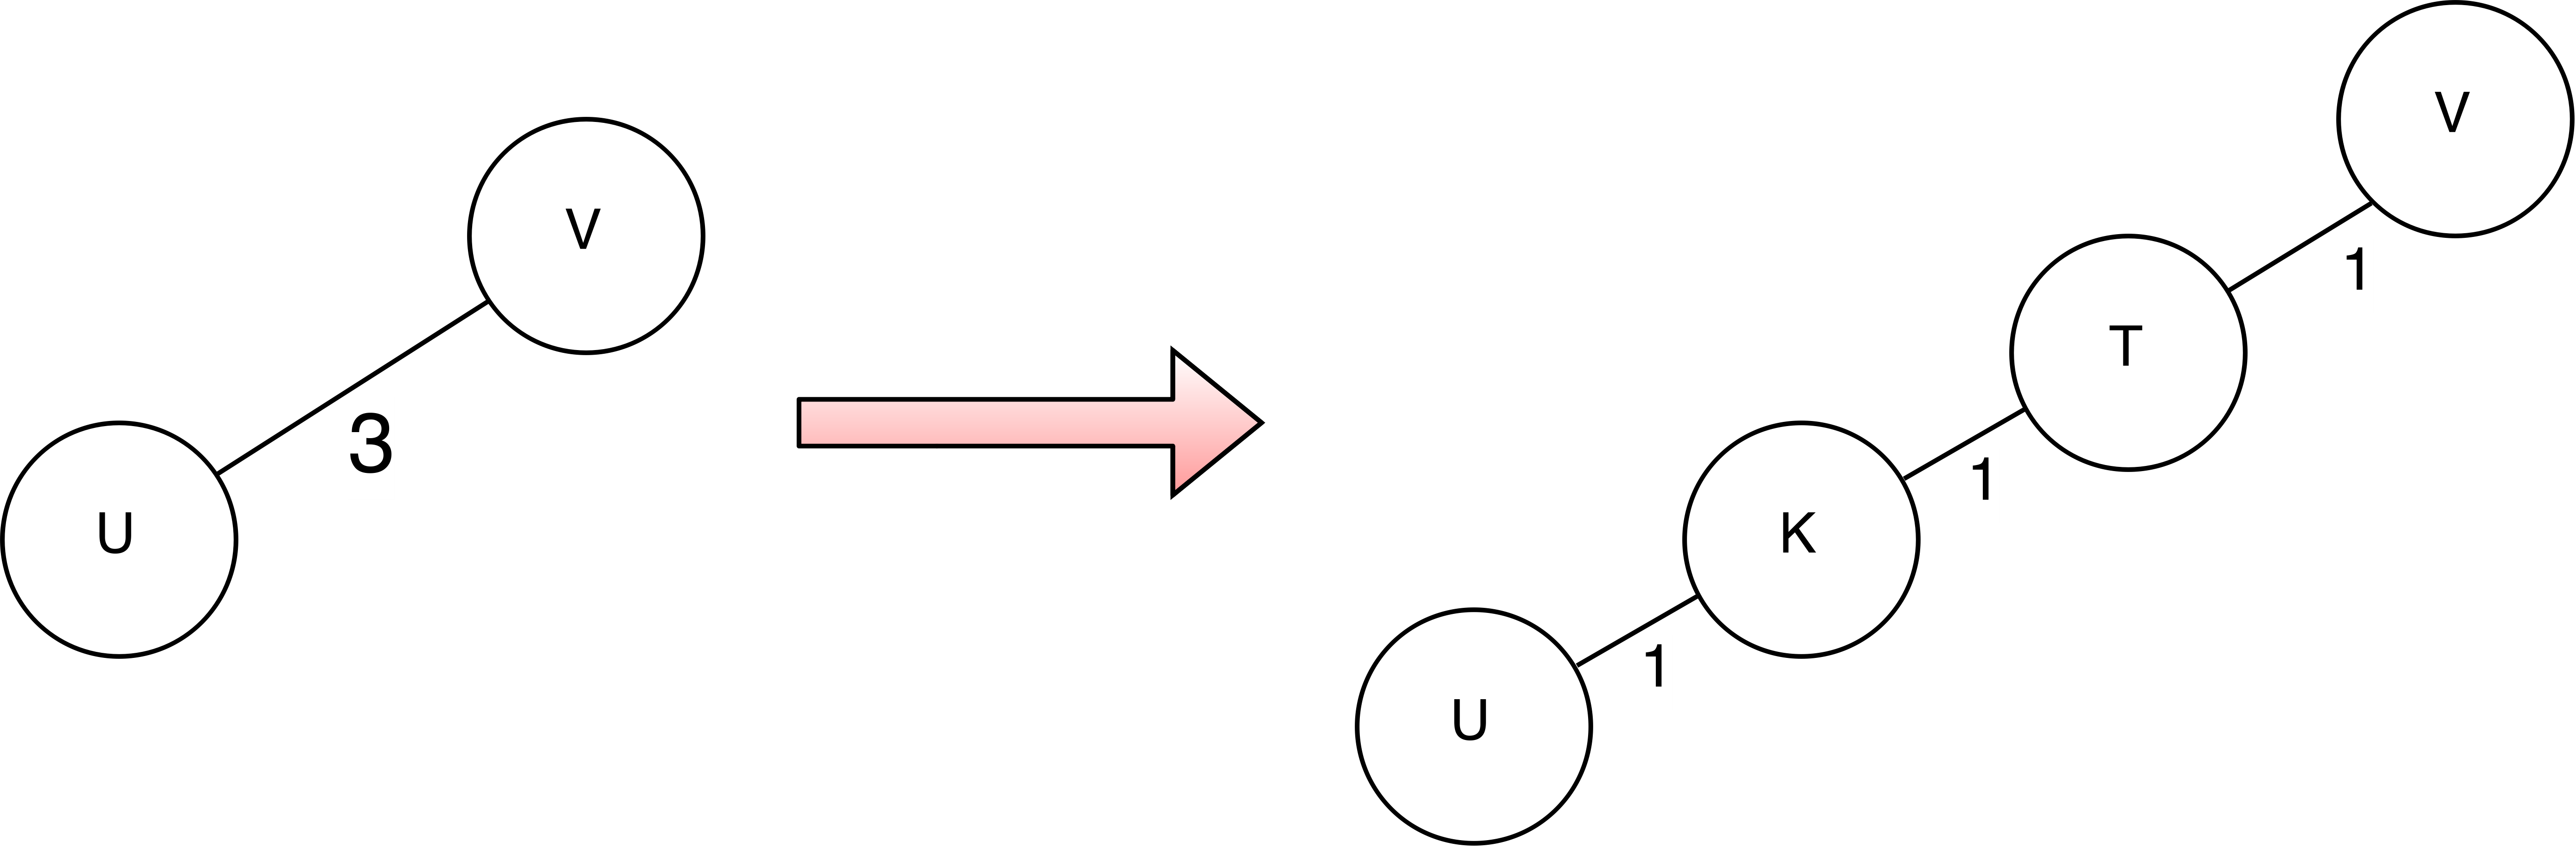
\includegraphics[width=0.9\textwidth]{img/floyd_social_modification.png}
\end{figure}
\FloatBarrier

В этой модификации алгоритм в худшем случае будет работать за $O(c \ VE)$ за счет увеличения числа ребер в $c$ раз.

\FloatBarrier
\section{Выводы}
Таким образом в этой части мы описали алгоритм для поиска кратчайшего расстояния на разреженных графах в общем случае (наивная версия) и для частного случая для социальных графов. При этом последний показал свою высокую эффективность на практике на реальных графах социальных сетей.
\FloatBarrier

%%-*-coding: utf-8-*-
\chapter{Сравнение с другими точными решениями}
\section{Модификация n-grid для точного решения}

В работе \cite{NGRID} была предложена структура данных n-grid, позволяющая
эффективно решать задачу поиска ближайшего отрезка. Автором этой работы
было предложено несколько алгоритмов фильтрации не ближайших отрезков из
ячеек сети. Но предложенные алгоритмы или осуществляют очень грубую
фильтрацию, оставляя при этом много лишних отрезков и не ухудшая точность
поиска ближайшего отрезка, или переходят к примерному решению задачи
поиска ближайшего отрезка, отфильтровывая возможно ближайшие отрезки.
Для этой структуры данных мной была применена та же схема
фильтрации, что и в квадродереве. После этого незначительного измения
данная структура данных позволила решать задачу поиска ближайшего отрезка
точно и оптимально, в смысле количества отрезков, которое нужно
рассматривать перебором

\section{Сравнительные испытания}

В сравнении будут участвовать:
\begin{itemize}
\item SVD (реализация из библиотеки CGAL);
\item модифицированный n-grid (модифицированная мною, реализация, используемая в компании
Транзас);
\item квадродерево (моя реализация).
\end{itemize}
Все испытания проводились на случайно генерируемых данных. Для
генерации данных бралась прямоугольная область пространства, в которой из
случайной точки этой области начинала генерироваться случайная цепь.
Случайная цепь характеризуется максимальной и минимальной длинами шага,
а также максимальным и минимальным углами поворота. При выходе цепи за
пределы области начинается генерация новой цепи. В результате получается
нечто, напоминающее картографические данные.

Для определения скорости поиска ближайшего отрезка производятся десять
тысяч случайных запросов.

В табл. \ref{query_time}, \ref{preproc_time}, \ref{mem_usage}, \ref{max_mem_usage}
приведены усредненные результаты сравнительных испытаний.

\begin{fasttable}{%
Скорость поиска ближайшего отрезка в миллисекундах
}{query_time}{
|r|r|r|r|
}
\hline
Алгоритм количество отрезков & 100 & 1000 & 10000 \\
\hline
n-grid   & 0,002725 & 0,002325 & 0,00198 \\
SVD      & 0,049175 & 0,047175 & 0,07255 \\
quadtree & 0,002375 & 0,002375 & 0,00195 \\
\hline
\end{fasttable}

\begin{fasttable}{%
Время препроцессирования в секундах
}{preproc_time}{
|r|r|r|r|
}
\hline
Алгоритм количество отрезков & 100 & 1000 & 10000 \\
\hline
n-grid   & 6,6535 & 87,5088 & 2256,4220 \\
SVD      & 0,0115 &  0,2425 &    5,2418 \\
quadtree & 1,6375 & 26,6068 &  488,0683 \\
\hline
\end{fasttable}

\begin{fasttable}{%
Количество памяти, занимаемой структурой, в мегабайтах
}{mem_usage}{
|r|r|r|r|
}
\hline
Алгоритм количество отрезков & 100 & 1000 & 10000 \\
\hline
n-grid   & 1,2233 &  2,0783 &   9,4328 \\
SVD      & 0,2200 &  1,0590 &   5,9438 \\
quadtree & 2,0423 & 12,5915 & 265,6437 \\
\hline
\end{fasttable}

\begin{fasttable}{%
Максимальное количество памяти, потребляемое при построении в мегабайтах
}{max_mem_usage}{
|r|r|r|r|
}
\hline
Алгоритм количество отрезков & 100 & 1000 & 10000 \\
\hline
n-grid   & 1,6870 &  8,7105 & 175,3023 \\
SVD      & 0,2200 &  1,0590 &   5,9438 \\
quadtree & 2,0423 & 12,5915 & 265,6437 \\
\hline
\end{fasttable}

Из результатов сравнения заметно, что многоуровневая сеть и
квадродерево работают на порядок быстрее, чем SVD. Время, затрачиваемое на
препроцессинг, и потребление памяти больше, но это цена за скорость работы.
Хоть квадродерево и потребляет больше памяти, чем многоуровневая сеть, но
при неравномерном распределении вершин диаграммы Вороного на плоскости
оно дает существенно лучшую скорость поиска ближайшего отрезка.
В таблице 5 приведены усредненные характеристики квадродеревьев,
полученных при испытаниях.
Характеристика\\количество отрезков
Количество ячеек
Среднее число отрезков в ячейке
Максимальная глубина
100
44
9,3
4
1000
596
12,5
7,25
Таблица 5 Усредненные характеристики квадродерева

%\chapter{Применение}
\section{Решение задачи обратного геокодирования}
Задача обратного геокодирования (reverse geocoding) состоит в
определении адреса по координатам точки.

Входными данными к этой задаче обычно является множество объектов
с известными географическими адресами. Поиск страны и некоторых других частей
адреса осуществляется за счет локализации в подразбиении карты мира на страны, 
страны на регионы и так далее. Для решения данной задачи известно множество методов.
Локализация на уровне улиц происходит иным образом. Определение улицы, рядом с 
которой расположена точка, осуществляется за счет поиска ближайшей улицы или дома (рис. \ref{rgeocoding}).

Эти данные представимы в виде отрезков, поэтому можно предобработать данные карты,
поместив геометрию карты в структуру для быстрого поиска ближайших отрезков, и запомнив
соответствие между геометрическими данными и их метаинформацией.

В результате, с помощью реализованного алгоритма, можно быстро решать задачу обратного геокодирования.

\drawfigure{rgeocoding}{Ближайший объект}{rgeocoding}

\FloatBarrier
\section{Решение задач интерполяции}
Быстрый поиск ближайших отрезков часто используется при интерполяции
функций, заданных на линейных объектах. Например, можно
восстанавливать высотную модель по изолиниям.

Также, зная расстояние до ближайшей линии, можно варьировать параметры
интерполяции. В работе \cite{NGRID} описано применение кампанией Транзас алгоритма
поиска ближайшего отрезка для восстановления рельефа по
картографическим данным. Они накладывают на известные данные шумы,
зависящие от расстояния до изолиний. Вблизи изолиний используется
высокочастотный шум низкой амплитуды, симулирующий мелкие неровности
рельефа, тогда как на удалении от них используется низкочастотный шум
большей амплитуды, позволяющий получать холмистую местность. Этот
подход позволяет по картографическим данным получать реалистичный
рельеф.

В этой же работе описано использование информации о ближайших отрезках
для простого текстурирования рельефа. В зависимости от расстояния до
линейных объектов применяются различные текстуры, которые плавно
переходят друг в друга. Например, в зависимости от расстояния до
береговой линии, сначала может идти текстура песка, а потом травяной растительности.

\FloatBarrier

%\startconclusionpage

Как было показано в данной работе, задача определение кратчайшего расстояния как от одной вершины, так и от множества может быть эффективна решена на нескольких вычислительных ядрах. Было предложено множество алгоритмов для нахождения расстояний, причем каждый из них имеет свои специфические особенности и рекомендации к применению на конкретных графах.

Параллельные алгоритмы из первой главы основаны на алгоритме Беллмана-Форда, который может быть использован в тех случаях, когда в графе присутствуют отрицательные ребра, циклы отрицательного веса или же когда заранее известно, что количество итерации будет невелико (как, например, в случае неориентированного невзвешенного графа алгоритм будет работать всего за $O(V + E)$). При этом, каждая из модификации оказалась лучше других на некоторых типа графах, что говорит о том, что после некоторого простого анализа входного графа мы можем выбрать наиболее оптимальный алгоритм для нашей ситуации.

В контексте параллельных алгоритмов поиска кратчайшего расстояния между каждой парой вершин был предложен алгоритм, идея которого была описана ранее (наивный алгоритм), а также предложена разработанная мною модификация для поиска расстояний на реальных социальных графах. Этот алгоритм оказался значительно быстрее наивной версии и может быть широко использован в подобных графов крупных социальных сетей, таких как Twitter, Facebook или Vkontakte. 

В предложенных алгоритмах использовались современные подходы и структуры данных для параллельных вычислений на графах (такие как Frontier), которые показали свою состоятельность и оказались заметно более эффективными по сравнению с предшествующими аналогами. Таким образом, есть все основания полагать, что подобные алгоритмы могут служить отличным эффективным решением для многопроцессорных архитектур с высоким количеством ядер.

\cite{FRONTIERSEARCH}
\cite{LIGRA}
\cite{CHUNKEDSEQ}
\cite{STANFORDGRAPHS}
\cite{CILK} 


\FloatBarrier


%\startappendices
%\label{appendix}
%\input{appendix}

\bibliography{thesis}

\end{document}
